% This file was created with tikzplotlib v0.10.1.
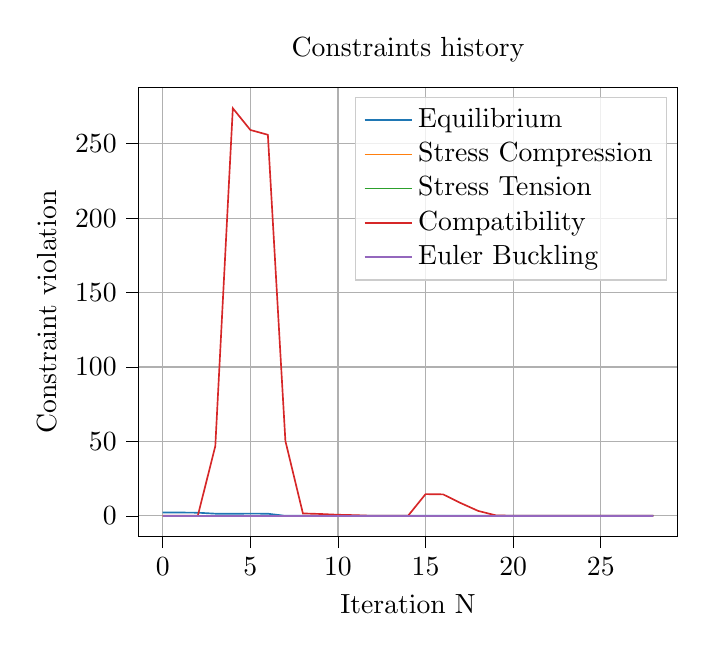
\begin{tikzpicture}

\definecolor{crimson2143940}{RGB}{214,39,40}
\definecolor{darkgray176}{RGB}{176,176,176}
\definecolor{darkorange25512714}{RGB}{255,127,14}
\definecolor{forestgreen4416044}{RGB}{44,160,44}
\definecolor{lightgray204}{RGB}{204,204,204}
\definecolor{mediumpurple148103189}{RGB}{148,103,189}
\definecolor{steelblue31119180}{RGB}{31,119,180}

\begin{axis}[
legend cell align={left},
legend style={fill opacity=0.8, draw opacity=1, text opacity=1, draw=lightgray204},
tick align=outside,
tick pos=left,
title={Constraints history},
x grid style={darkgray176},
xlabel={Iteration N},
xmajorgrids,
xmin=-1.4, xmax=29.4,
xtick style={color=black},
xtick={-5,0,5,10,15,20,25,30},
xticklabels={
  \(\displaystyle {\ensuremath{-}5}\),
  \(\displaystyle {0}\),
  \(\displaystyle {5}\),
  \(\displaystyle {10}\),
  \(\displaystyle {15}\),
  \(\displaystyle {20}\),
  \(\displaystyle {25}\),
  \(\displaystyle {30}\)
},
y grid style={darkgray176},
ylabel={Constraint violation},
ymajorgrids,
ymin=-13.6892178194271, ymax=287.473574207968,
ytick style={color=black},
ytick={-50,0,50,100,150,200,250,300},
yticklabels={
  \(\displaystyle {\ensuremath{-}50}\),
  \(\displaystyle {0}\),
  \(\displaystyle {50}\),
  \(\displaystyle {100}\),
  \(\displaystyle {150}\),
  \(\displaystyle {200}\),
  \(\displaystyle {250}\),
  \(\displaystyle {300}\)
}
]
\addplot [semithick, steelblue31119180]
table {%
0 2.21099398489335
1 2.21099398489335
2 2.09311104367434
3 1.4408158696362
4 1.35135435932169
5 1.50109059263075
6 1.40445487395147
7 0.0054914603954046
8 0.000262286588878169
9 6.18125426399274e-08
10 4.75987007000823e-09
11 4.15099066231051e-11
12 1.06105361421261e-13
13 1.06105361421261e-13
14 9.31734689402219e-10
15 4.00092829977439e-08
16 1.29277367477698e-07
17 9.03556554021634e-08
18 4.00015665036335e-08
19 1.63877206685754e-08
20 4.01358716265932e-09
21 2.26144623052483e-10
22 1.85474469953785e-11
23 9.50277216138802e-14
24 2.8421709430404e-14
25 1.4210854715202e-14
26 1.4210854715202e-14
27 1.42169232471728e-14
28 7.1055280068803e-15
};
\addlegendentry{Equilibrium}
\addplot [semithick, darkorange25512714]
table {%
0 0
1 0
2 0
3 0
4 0
5 0
6 0
7 0
8 0
9 0
10 0
11 0
12 0
13 0
14 0
15 0
16 0
17 0
18 0
19 0
20 0
21 0
22 0
23 0
24 0
25 0
26 0
27 0
28 0
};
\addlegendentry{Stress Compression}
\addplot [semithick, forestgreen4416044]
table {%
0 0
1 0
2 0
3 0
4 0
5 0
6 0
7 0
8 0
9 0
10 0
11 0
12 0
13 0
14 0
15 0
16 0
17 0
18 0
19 0
20 0
21 0
22 0
23 0
24 0
25 9.19393983167538e-09
26 9.99801841317094e-09
27 9.99798999146151e-09
28 9.99801841317094e-09
};
\addlegendentry{Stress Tension}
\addplot [semithick, crimson2143940]
table {%
0 1.13249143396388e-09
1 1.13249143396388e-09
2 0.006205803418041
3 46.8297443105993
4 273.784356388541
5 259.207310268827
6 255.957163295949
7 50.3175679384794
8 1.60067445608256
9 1.24111658126421
10 0.713742825334293
11 0.431186031427671
12 0.0100868971508135
13 0.0100868971508135
14 0.0108775115787694
15 14.5709169215562
16 14.4164018214648
17 8.61321411517599
18 3.30280055206103
19 0.334024137240441
20 0.0235816512459763
21 7.57655090808385e-05
22 9.89223479876955e-05
23 9.81095338943305e-05
24 9.99040972899934e-05
25 0.000100009156220437
26 0.000100009997986206
27 0.000100009997986206
28 0.000100009997993311
};
\addlegendentry{Compatibility}
\addplot [semithick, mediumpurple148103189]
table {%
0 0
1 0
2 0
3 0
4 0
5 0
6 0
7 0
8 0
9 0
10 0
11 0
12 0
13 0
14 0
15 0
16 0
17 0
18 0
19 0
20 0
21 0
22 0
23 0
24 0
25 0
26 0
27 0
28 0
};
\addlegendentry{Euler Buckling}
\end{axis}

\end{tikzpicture}
